\begin{thema}{Β}
Δίνεται η συνάρτηση $f(x) = x \ln x - x + 1$.

\begin{erwthma}
\item Πρέπει $x > 0$. Άρα $D_f = (0, +\infty)$.
Για το όριο $\lim\limits_{x \to 0^+} f(x)$, υπολογίζουμε το όριο $\lim\limits_{x \to 0^+} (x \ln x)$. 

\begin{align*}
\lim\limits_{x\to 0^+}{(x\ln{x})}&\xlongequal{0\cdot(-\infty)}\lim\limits_{x\to 0^+}{\frac{\ln{x}}{\frac{1}{x}}}\dlh{\frac{-\infty}{+\infty}}\lim\limits_{x\to 0^+}{\frac{\frac{1}{x}}{-\frac{1}{x^2}}}=\lim\limits_{x\to 0^+}{(-x)}=0
\end{align*}

Επομένως:
\[ \lim_{x\to0^+} f(x) = \lim_{x\to0^+} (x \ln x - x + 1) = 0 - 0 + 1 = 1 \]

\item Η $f$ είναι παραγωγίσιμη στο $(0, +\infty)$ με:
\[ f'(x) = (x\ln x)' - (x)' + (1)' =  1 \cdot \ln x + x \cdot \frac{1}{x}  - 1 = \ln x + 1 - 1 = \ln x \]
Έχουμε 
\begin{itemize}
\item $f'(x) = 0 \Leftrightarrow \ln x = 0 \Leftrightarrow x = 1$.
\item $f'(x) > 0 \Leftrightarrow \ln x > 0 \Leftrightarrow x > 1$, και 
\item $f'(x) < 0 \Leftrightarrow 0 < x < 1$.
\end{itemize}

Στον παρακάτω πίνακα φαίνεται το πρόσημο της $f'$ και η μονοτονία της $f$:
\begin{center}
\begin{tikzpicture}
\tkzTabInit[color,lgt=2,espcl=1.5,colorC = red7,colorL = red9,colorV = red7]%
{$x$ / .8,$f'(x)$ /0.8,$f(x)$/0.8}%
{$0$,$1$,$+\infty$}%
\tkzTabLine{ d, -, z, +, }
\tkzTabVar{ D+/,-/{\tiny OE},+/, }
\end{tikzpicture}
\end{center}
Η $f$ παρουσιάζει ολικό ελάχιστο στο $x_0 = 1$ με τιμή $f(1) = 1\ln 1 - 1 + 1 = 0$.

\item Από το προηγούμενο ερώτημα δείξαμε ότι το ολικό ελάχιστο της $f$ είναι το $0$. Επομένως για κάθε $x > 0$:
\[ f(x) \ge 0 \Leftrightarrow x \ln x - x + 1 \ge 0 \Leftrightarrow x \ln x \ge x - 1 \]
με την ισότητα να ισχύει μόνο για $x = 1$.

\item Στο διάστημα $[1, e]$, ξέρουμε ότι $f(x) \ge 0$. Άρα το εμβαδόν είναι:
\[ E = \int_1^e f(x) dx = \int_1^e (x \ln x - x + 1) dx \]
Υπολογίζουμε πρώτα με παραγοντική το ολοκλήρωμα $\int_1^e x \ln x dx$:
\[ \int_1^e x \ln x dx = \int_1^e \left(\frac{x^2}{2}\right)' \ln x dx = \left[ \frac{x^2}{2} \ln x \right]_1^e - \int_1^e \frac{x^2}{2} \cdot \frac{1}{x} dx \]
\[ = \frac{e^2}{2} \ln e - \frac{1^2}{2} \ln 1 - \frac{1}{2}\int_1^e x dx = \frac{e^2}{2} - \frac{1}{2} \left[ \frac{x^2}{2} \right]_1^e = \frac{e^2}{2} - \frac{e^2}{4} + \frac{1}{4} = \frac{e^2+1}{4} \]
Στη συνέχεια υπολογίζουμε το υπόλοιπο κομμάτι:
\[ \int_1^e (-x+1) dx = \left[ -\frac{x^2}{2} + x \right]_1^e = \left(-\frac{e^2}{2} + e\right) - \left(-\frac{1}{2} + 1\right) = -\frac{e^2}{2} + e - \frac{1}{2} \]
Συνολικά έχουμε:
\[ E = \frac{e^2+1}{4} - \frac{2e^2}{4} + \frac{4e}{4} - \frac{2}{4} = \frac{-e^2 + 4e - 1}{4} \]
\end{erwthma}
\end{thema}
